% 中文精修稿；底本为 core_zh_initial.tex，英文快照为 core_translation_source.tex。
% 主文件提供中文排版支持、amsmath、amssymb、amsthm 及 theorem/lemma/proof 环境。
% 翻译与精修记录见 core_zh_sentence_audit.md；本文仍处于独立核验前的草稿阶段。

\section{星形 Kakeya 集的十分之一面积下界}
\label{sec:core-tenth}

% [E01]
星形集包含一条单位线段，就必然包含相应的三角形。把星形中心放在原点，取端点为 $(-1/2,h)$ 和 $(1/2,h)$ 的水平线段。原点与这条底边上任一点之间的线段都属于该集合，因此整个三角形都属于它。三角形的面积是 $|h|/2$。底边到原点的距离只要至少为 $1/5$，就得到了所求下界。

% [E02]
困难出现在每条选定的底边都靠近原点的情形。若 $h\ne0$，以原点为中心旋转整条底边及其三角形，就得到另一个同面积的三角形；底边的中点也随之转动。两者的内部会重叠：第一个三角形的内点在充分小的旋转之后仍然是内点。直接相加两个三角形的面积，会把重叠部分计算两次。另一种极端情形是 $h=0$：若取以原点为中点的线段的所有旋转，每个三角形的面积都为零，并集却是半径为 $1/2$ 的圆盘。这两个例子都要求我们测量并集本身。我们沿同心圆测量这个并集；每个三角形的截面至多由两个实际角度区间组成。

\begin{theorem}
\label{thm:core-tenth}
设 $E\subseteq\mathbb R^2$，且存在一点 $o\in\mathbb R^2$，使得对每个 $x\in E$ 都有 $[o,x]\subseteq E$。再设每个无向方向 $q\in\mathbb {RP}^1$ 上都有一条沿方向 $q$、长为一的闭线段包含在 $E$ 中。那么 $E$ 的 Lebesgue 外测度满足
\[
                 |E|^*\geq\frac1{10}.
\]
\end{theorem}

% [E03]
这个命题适用于平面的任意子集和任意星形中心。因此，证明必须自行构造可测对象，不能假设能从 $E$ 中可测地选出各方向的线段。得到可测族后，只要近端点离中心足够远，主要的几何估计就同时使用两个端点。近端点半径较小的方向则有半径更大的远端点，可以在更大的半径上补足贡献。我们在半径为 $1/2$ 的圆盘内平衡这两种贡献，再用互不相交的圆环处理其余方向。

\subsection{在开覆盖内重新选取可测三角形族}
\label{subsec:core-recovery}

% [R01]
把 $o$ 平移到 $0$，并任取一个开集 $G\supseteq E$。只需对每个这样的 $G$ 证明 $|G|\geq1/10$，因为 Lebesgue 外测度等于所有开超集测度的下确界。对每个方向 $q$，从 $E$ 中选出一条单位线段，记其端点为 $A_q,B_q$，并令
\[
                  T_q=\operatorname{conv}\{0,A_q,B_q\}.
\]
$T_q$ 中的每一点都位于 $0$ 与 $[A_q,B_q]$ 上某一点之间的线段上，所以 $T_q\subseteq E\subseteq G$。

% [R02]
暂时允许这些选择任意依赖于 $q$。这里采用与开头整体旋转不同的操作：固定一个选定三角形的底边中点，仅改变底边方向。不区分端点次序时，线段及三角形都随方向在 Hausdorff 距离下连续变化。这里的 Hausdorff 连续性指双向的逐点接近。对两次放置中用同一局部角度坐标匹配的端点，保持凸组合系数不变，所得三角形点的位移至多为两个端点位移的最大值；反向匹配也有同一估计。原三角形是开集 $G$ 内的紧集，因此充分小的变化仍留在 $G$ 中。于是，同一个中点在原方向的一个开邻域内都可使用。这些邻域覆盖紧圆周 $\mathbb {RP}^1$；从中取有限子覆盖 $O_1,\ldots,O_k$，相应中点记为 $c_1,\ldots,c_k$。

% [R03]
将 $q$ 分配给第一个包含它的 $O_j$，并用 $c_j$ 作为相应线段的中点。各集合 $O_j\setminus\bigcup_{i<j}O_i$ 都是 Borel 集，因此这给出了一个 Borel 中点选择。方向仍遍历整个射影圆周；有限的只是中点取值的列表。每个新三角形都包含在 $G$ 内，但它的底边未必属于原集合 $E$。以下用 $A_q,B_q,T_q$ 表示重新选出的对象。

% [R04]
下文需要一个可测性事实。完备可分度量空间中 Borel 子集的 Borel 像称为解析集。在本文的欧氏空间和角度空间中，解析集以及 Borel 集的投影都是 Lebesgue 可测的。这是本证明所需的可测投影定理。对一个 Borel 方向集 $V$，令
\begin{align*}
 W(V)&=\bigcup_{q\in V}T_q,\qquad W=W(\mathbb {RP}^1),\\
 S_r(V)&=\{\theta\in\mathbb R/(2\pi\mathbb Z):
                  r(\cos\theta,\sin\theta)\in W(V)\},\quad r>0.
\end{align*}
取 $q\in[0,\pi)$ 作为无向方向的实角度代表，固定 $u_q=(\cos q,\sin q)$ 和逆时针法向 $n_q=(-\sin q,\cos q)$。已选中点 $c(q)$ 是 Borel 映射，所以明确规定 $A_q=c(q)-u_q/2$、$B_q=c(q)+u_q/2$ 就得到两个 Borel 端点映射。映射
\[
 (q,a,b)\longmapsto aA_q+bB_q,
 \qquad a,b\geq0,\quad a+b\leq1,
\]
是 Borel 映射，在 $q\in V$ 时的像恰为 $W(V)$，故 $W(V)$ 是解析集。它的联合极坐标关联集
\[
 \{(r,\theta):r>0,\ r(\cos\theta,\sin\theta)\in W(V)\}
\]
也是解析集：在上式的等式中引入 $q,a,b$，再将所得 Borel 集投影即可。固定 $r$ 后用同样的论证，可知每个 $S_r(V)$ 都可测。因此，可以对实际并集使用极坐标积分与 Tonelli 定理，证明中所用的所有子族也都如此。
下文所说的 Borel 族，是指在一个 Borel 方向集上每个方向恰有一条单位线段，且端点映射为 Borel 映射；子族通过限制这些相同的映射得到。

% [R05]
在正交单位坐标下，将重新选出的线段写成
\[
 A=(s-1/2)u+h n,\qquad B=(s+1/2)u+h n,
\]
其中 $u$ 是其方向的 Borel 单位代表，$n$ 是将其旋转四分之一周所得的向量。若重新选出的任意一条线段满足 $|h|\geq1/5$，其三角形就包含于 $G$ 且面积至少为 $1/10$。因此，以下可对重新选出的族假设
\begin{equation}
                    |h(q)|<1/5\quad\hbox{对每个 }q.
\label{eq:core-height}
\end{equation}
这个分情形步骤必须放在重新选取之后。固定中点 $c_j$ 时，它的位置和范数不变，但相对于底边法向的分量 $h(q)=c_j\cdot n_q$ 可能随方向改变。

\subsection{实际角度、并集与单侧延伸估计}
\label{subsec:core-intervals}

% [I01]
无向方向组成一个长度为 $\pi$ 的圆周，实际角度则组成一个长度为 $2\pi$ 的圆周。两者都使用通常的长度测度，方向长度记为 $|V|$，实际角度长度记为 $|S|$。从实际角度到方向的映射将对径点认作同一点。对每个 $q\in V$，以 Borel 方式从它的两个提升中选择一个，所得角度集的长度是 $|V|$，而非 $2|V|$。具体地，以角度模 $\pi$ 表示无向方向，在坐标区间 $[0,\pi)$ 上用 Borel 函数 $\chi:V\to\{0,1\}$ 记录所选的一侧，提升就是 $q\mapsto q+\pi\chi(q)$。$\chi=0$ 和 $\chi=1$ 两部分的像落在不同的半圆上，后者只是平移 $\pi$，故两像的长度之和恰为 $|V|$。

% [I02]
区分这两个圆周后，就可以比较理想方向和实际圆弧。从原点看去，底边端点所在的方向未必就是底边自身的方向。我们把端点的实际角度区间延伸到这个理想方向，并控制整个并集增加的长度。下面的初等估计允许任意重叠、重复区间，以及向任一侧延伸。

\begin{lemma}[并集的单侧延伸]
\label{lem:core-interval}
设 $(J_i)_{i\in I}$ 是任意一族闭圆周区间，允许单点区间。固定 $\rho\geq0$，将每个 $J_i$ 的一端延长至多 $\rho|J_i|$，得到 $K_i$。则
\begin{equation}
 \left|\bigcup_{i\in I}K_i\right|^*
       \leq(1+2\rho)\left|\bigcup_{i\in I}J_i\right|^*.
\label{eq:core-interval}
\end{equation}
\end{lemma}

\begin{proof}
% [I03]
取包含 $\bigcup_iJ_i$ 的开圆周集 $O$。若 $O$ 是整个圆周，它的测度已经给出了延伸后并集所需的上界。否则，$O$ 是可数个互不相交开弧的并。由于 $J_i$ 连通，它必包含在某个长为 $\ell$ 的连通分支 $C$ 中，且 $|J_i|\leq\ell$。将 $C$ 的两端各延伸 $\rho\ell$，就包含了所有对应的 $K_i$；即使延伸后绕过整圈，其圆周长度也至多为 $(1+2\rho)\ell$。这些扩大的分支覆盖延伸后的并集。先用测度对可数并的次可加性，再对 $O$ 取下确界，就得到 \eqref{eq:core-interval}。

% [I04]
单点区间的长度为零，因此只能作零长度延伸。上面的证明仍适用于不可数的单点族，它们的并集可能具有正长度。重复出现的非退化基区间也只通过它们的并集进入右端，即使它们分别向相反方向延伸也是如此。
\end{proof}

% [I05]
径向积分将使用测度
\begin{equation}
 d\nu(x)=\min\{1,|x|^{-1}\}\,dx
        =\min\{r,1\}\,dr\,d\theta,
\label{eq:core-nu}
\end{equation}
其在 $0$ 处的密度定义为 $1$。因此，$\nu$ 在单位圆盘内等于通常面积，在外部也不超过通常面积。对每个非负 Borel 函数 $p$，都有
\begin{equation}
 \int_{W(V)}p(|x|)\,d\nu(x)
     =\int_0^\infty p(r)\min\{r,1\}|S_r(V)|\,dr.
\label{eq:core-polar}
\end{equation}
函数 $p$ 指定估计在各半径处使用的面积比例。若若干子并集互相重叠，只要它们的加权示性函数之和不超过 $1_W$，就可以相加其贡献。这是对实际点逐点施加的条件，而不是对方向标签施加的条件。

\subsection{以原点为顶点的三角形的完整截面}
\label{subsec:core-sections}

% [G01]
让每条底边朝向离原点最远的端点。具体地，若 $|B_q|\geq|A_q|$ 就沿 $u_q$，否则沿 $-u_q$，并把局部法向也同时反向。其提升选择函数正是 $\chi(q)=\mathbf1_{\{|A_q|>|B_q|\}}$，一个 Borel 函数；等长时固定选择 $B_q$。在相应局部坐标下，两个端点为
\begin{equation}
 (x-1,h),\quad(x,h),\qquad x\geq1/2,
 \qquad z=|h|,\quad
 M^2=x^2+z^2,\quad N^2=(x-1)^2+z^2.
\label{eq:core-endpoints}
\end{equation}
这里 $M$ 和 $N$ 分别是较大和较小的\emph{端点}半径。整个三角形也位于半径为 $M$ 的闭圆盘内：对非负的凸组合系数 $a,b$，$a+b\leq1$ 给出 $|aA_q+bB_q|\leq(a+b)M\leq M$。两个端点半径的平方之差为 $2x-1$，这就说明了为何 $x\geq1/2$。单位底边还给出
\begin{equation}
                         M+N\geq1,\qquad M\geq1/2.
\label{eq:core-unit}
\end{equation}
线段上最近点的半径，在 $x\leq1$ 时为 $z$，在 $x>1$ 时为 $N$。必须区分这两种情形，因为圆周可能不与底边相交，却仍切过填满的三角形。

% [G02]
先设 $z>0$，朝底边实际所在的一侧测量局部角度 $\phi$。令
\[
 b=\arctan(z/x),\qquad d=\operatorname{atan2}(z,x-1),\qquad
 \gamma=d-b.
\]
角度 $d\in(0,\pi)$ 是较近端点在这些坐标下的辐角；这里的两变量记法明确表示
\[
 d=\begin{cases}
 \arctan\bigl(z/(x-1)\bigr),&x>1,\\
 \pi/2,&x=1,\\
 \pi-\arctan\bigl(z/(1-x)\bigr),&x<1.
 \end{cases}
\]
三角形占据角域 $[b,d]$。角域内的射线在半径 $z/\sin\phi$ 处与底边相交，三角形包含这条射线上所有更小的半径。因此，其半径为 $r$ 的完整截面在这些坐标下为
\begin{equation}
 S_r(T_q)=
 \begin{cases}
 [b,d],&0<r\leq z,\\[2pt]
 [b,d]\cap\bigl([0,a_r]\cup[\pi-a_r,\pi]\bigr),
       &r>z,\quad a_r=\arcsin(z/r).
 \end{cases}
\label{eq:core-full-section}
\end{equation}
对于 $h<0$，将这些局部区间放回原平面中有向底边的另一侧即可。这只是同一个三角形的坐标描述，并未向 $W$ 添加反射后的三角形。

% [G03]
当 $1/2\leq x<1$ 时，垂足严格落在底边内部，且 $d>\pi/2$。在 $r>z$ 时，截面可能有两个分支，各靠近一个端点。若 $r<M$，远端分支恰为 $[b,a_r]$；若 $r<N$，近端分支恰为 $[\pi-a_r,d]$。在 $r=z$ 时，两部分相接，仍得到完整角域。当 $x>1$ 时，两端点位于纵向的同一侧，且 $d<\pi/2$。对 $z<r<N$，有 $a_r>d$，因此即使底边不与半径为 $r$ 的圆周相交，整个角域仍然存在。对 $N<r<M$，角域缩为 $[b,a_r]$。在 $x=1$ 时，垂足是一个端点且 $d=\pi/2$，同一公式也包含这一情形。

% Illustrative exact-coordinate unit triangle; no numerical-search result.
% Requires tikz and decorations.pathreplacing.
\begin{figure}[tb]
\centering
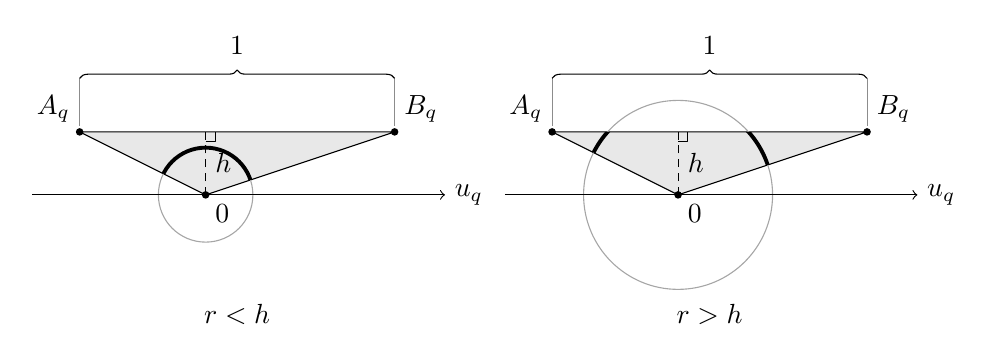
\begin{tikzpicture}[x=4cm,y=4cm,line join=round]
\foreach \rad/\shift/\tag in {0.15/0/{r<h},0.30/6/{r>h}} {
 \begin{scope}[xshift=\shift cm]
  \coordinate (O) at (0,0);
  \coordinate (Far) at (0.6,0.2);
  \coordinate (Near) at (-0.4,0.2);
  \fill[black!9] (O)--(Far)--(Near)--cycle;
  \draw[thin] (O)--(Far)--(Near)--cycle;
  \draw[black!35] (O) circle (\rad);
  \begin{scope}
   \clip (O)--(Far)--(Near)--cycle;
   \draw[line width=1.4pt] (O) circle (\rad);
  \end{scope}
  \draw[densely dashed] (O)--(0,0.2) node[midway,right] {$h$};
  \draw[thin] (0,0.17)--(0.03,0.17)--(0.03,0.2);
  \draw[->,thin] (-0.55,0)--(0.76,0) node[right] {$u_q$};
  \draw[black!45,thin] (-0.4,0.22)--(-0.4,0.37) (0.6,0.22)--(0.6,0.37);
  \draw[decorate,decoration={brace,amplitude=3pt}] (-0.4,0.37)--(0.6,0.37)
    node[midway,above=5pt] {$1$};
  \fill (O) circle (0.012) node[below right] {$0$};
  \fill (Far) circle (0.012) node[above right] {$B_q$};
  \fill (Near) circle (0.012) node[above left] {$A_q$};
  \node at (0.10,-0.38) {$\tag$};
 \end{scope}
}
\end{tikzpicture}
\caption{同一完整单位针在两个半径上的截面。浅色是原点三角形，粗圆弧是它的实际圆周截面。左图的圆周尚未达到底边，远端和近端使用同一完整角域；右图的圆周跨过底边后，截面分成两条端部弧。对两个端点计数，不意味着可以将左图的同一条粗弧计算两次。}
\label{fig:needle-sections}
\end{figure}


% [G04]
特别地，对每个 $0<r<M$，都有一个实际的远端基区间
\begin{equation}
 J_r(q)=
 \begin{cases}
 [b,d],&r\leq z,\\
 [b,\min\{d,a_r\}],&z<r<M.
 \end{cases}
\label{eq:core-far-base}
\end{equation}
第二种情形下，它的长度为 $\min\{\gamma,a_r-b\}$。这个最小值保证了垂足落在底边外时，区间仍处于实际角域之内。将此基区间向角度 $0$ 延伸，只需增加长度 $b$，便到达底边的理想远端方向。

% [G05]
若 $z=0$，三角形就是从 $0$ 到 $x$ 的径向区间；在 $x<1$ 时，还包含反方向长为 $1-x$ 的径向区间。对 $0<r<M=x$，取实际远端射线在圆周上的单点作为基区间。它已与理想远端锚点重合，无需延伸。上述径向区间均为闭区间，所以在 $r=M$ 时仍保留远端方向的单点；存在反向径向区间时，其正半径端点也被保留。这类方向可能构成方向测度为正的集合，因此下文每个并集估计都保留它们。

\begin{lemma}[远端截面下界]
\label{lem:core-far}
设一个 Borel 单位线段族满足 $M\geq m\geq1/2$。再设存在固定的有限常数 $B\geq0$，使其中所有 $z>0$ 的成员都满足 $b/\gamma\leq B$。那么，该族的每个 Borel 方向子集 $V$ 都满足
\begin{equation}
 |S_r(V)|\geq
 \min\left\{\frac1{1+2B},\frac{m-r}{m+r}\right\}|V|,
                   \qquad 0<r<m.
\label{eq:core-far-kernel}
\end{equation}
\end{lemma}

\begin{proof}
% [G06]
对 $0<t\leq1$，比值 $\arcsin(t)/t$ 单调递增，因为它是递增函数 $(1-v^2)^{-1/2}$ 在 $[0,t]$ 上的平均值。若 $z<r<M$，则 $b=\arcsin(z/M)$，因而
\[
 \frac{b}{a_r}\leq\frac rM,\qquad
 \frac{b}{a_r-b}\leq\frac r{M-r}\leq\frac r{m-r}.
\]
对实际基区间 \eqref{eq:core-far-base}，延伸长度与基区间长度之比因此不超过
\[
                   \rho=\max\{B,r/(m-r)\}.
\]
分母取两个候选长度的最小值，所得比值就是相应两个比值的最大值；完整角域情形下，比值不超过 $B$。零高度的单点区间也满足这一延伸条件。

% [G07]
对所有这些实际基区间一次性应用引理~\ref{lem:core-interval}。它们的并集包含于 $S_r(V)$，延伸后的并集则包含 $V$ 中每个方向的一个按 Borel 规则选出的理想远端提升。这个提升集的长度为 $|V|$，所以
\[
                  |V|\leq(1+2\rho)|S_r(V)|.
\]
取 $1+2\rho$ 的倒数，就得到 \eqref{eq:core-far-kernel}。这一次应用已经同时处理了正、负高度，完整角域、较短的端部弧，以及它们在平面中的所有重叠。
\end{proof}

\begin{lemma}[由端点半径上界控制角域]
\label{lem:core-bounded}
设
\[
 0<H\leq1/2,\qquad m\geq1/2,\qquad
 R\geq\max\{m,\sqrt{1/4+H^2}\},
\]
且一个 Borel 族满足 $m\leq M\leq R$ 和 $|h|\leq H$。那么，对每个 Borel 方向子集 $V$ 及 $0<r<m$，都有
\begin{equation}
 |S_r(V)|\geq
 \min\left\{K(R,H),\frac{m-r}{m+r}\right\}|V|,
 \qquad
 K(R,H)=\frac{\sqrt{R^2-H^2}}{\sqrt{R^2-H^2}+2R^2}.
\label{eq:core-bounded-kernel}
\end{equation}
\end{lemma}

\begin{proof}
% [G08]
对 $z>0$，角域张角为
\[
 \gamma=\int_{x-1}^{x}\frac{z}{t^2+z^2}\,dt.
\]
由于 $x\geq1/2$，每个 $t\in[x-1,x]$ 都满足 $|t|\leq x$。于是 $\gamma\geq z/M^2$；再由 $b\leq z/x$ 得
\[
                     \frac b\gamma\leq\frac{M^2}{x}
                                           =x+\frac{z^2}{x}.
\]
固定 $z\leq H\leq1/2$ 后，最后一个表达式在 $x\geq1/2$ 上递增，因为它的导数为 $1-z^2/x^2\geq0$。约束 $M\leq R$ 给出 $x\leq\sqrt{R^2-z^2}$，故
\[
 \frac b\gamma\leq\frac{R^2}{\sqrt{R^2-z^2}}
                  \leq\frac{R^2}{\sqrt{R^2-H^2}}.
\]
用这个 $B$ 值应用引理~\ref{lem:core-far} 即可。假设保证了各分母为正，也保证了放宽后的 $(x,z)$ 定义域中所用的上端点可行。这个积分论证同时包含垂足在底边内部和外部的情形。
\end{proof}

\subsection{在内圆盘中使用满足条件的近端点}
\label{subsec:core-low}

% [L01]
将满足 $M<99/100$ 的方向称为低半径方向，记它们组成的 Borel 集为 $L$。在 $L$ 上，式~\eqref{eq:core-endpoints} 给出 $1/2\leq x<1$，所以每条底边都跨过自己的垂足。固定任意 Borel 子集 $V\subseteq L$，将它分成
\begin{equation}
 B(V)=\{q\in V:N(q)\geq2/5\},\qquad U(V)=V\setminus B(V).
\label{eq:core-eligible-split}
\end{equation}
对 $V$ 的每个方向都选取远端点，并且仅在 $B(V)$ 上再选取近端点。每个被选端点的半径都至少为 $2/5$。虽然各端点半径随方向变化，这个共同阈值仍允许我们只作一次延伸估计。

\begin{lemma}[可选端点给出的下界]
\label{lem:core-eligible}
对每个 Borel 子集 $V\subseteq L$ 及 $0<r<2/5$，都有
\begin{equation}
 |S_r(V)|\geq k_4(r)\bigl(|V|+|B(V)|\bigr),\qquad
 k_4(r)=\min\left\{\frac23,\frac{2/5-r}{2/5+r}\right\}.
\label{eq:core-eligible}
\end{equation}
\end{lemma}

\begin{proof}
% [L02]
先控制将完整角域延伸到选定锚点所需的长度。对 $z>0$，记
\[
 b=\arctan(z/x),\quad c=\arctan\bigl(z/(1-x)\bigr),\quad
 \gamma=\pi-b-c.
\]
实际角域为 $[b,\pi-c]$。向远端和近端延伸，分别需要长度 $b$ 和 $c$。我们断言，整个低半径族都满足 $b/\gamma<1/4$，包括那些近端点未被选取的方向。

% [L03]
固定 $0<z\leq1/5$，只需证明 $5b+c<\pi$。若 $1/2\leq x\leq4/5$，则
\[
 b\leq z/x\leq2/5,\qquad
 c=\arctan\bigl(z/(1-x)\bigr)\leq\arctan1=\pi/4,
\]
故 $5b+c\leq2+\pi/4<\pi$。若 $4/5<x<1$，则
\[
 b\leq z/x\leq1/4,\qquad c<\pi/2,
\]
从而 $5b+c<5/4+\pi/2<\pi$。这两种情况都只用了非负参数上的 $\arctan t\leq t$、反正切的单调性和 $\pi>3$。于是 $4b<\pi-b-c=\gamma$，证明了远端的四分之一延伸界，不要求近端点可选。

若近端点被选取，则 $M\geq N\geq2/5$，因此
\[
 \sin b=z/M\leq1/2,\qquad \sin c=z/N\leq1/2.
\]
两个角都在 $(0,\pi/2)$ 内；由该区间上正弦的严格单调性和 $\sin(\pi/6)=1/2$，得 $b,c\leq\pi/6$。因而 $\gamma\geq2\pi/3$ 且 $c/\gamma\leq1/4$。这后一条界只用于近端点确实可选的方向。

% [L04]
现在固定 $r\in(0,2/5)$。对满足 $r\leq z$ 的成员，将整个角域作为每个选定端点的实际基区间。若两端点都被选取，就把同一个角域列出两次，分别向两侧延伸；每次都至多延伸基区间长度的四分之一。对满足 $0<z<r$ 的成员，令 $a=\arcsin(z/r)$。选定的实际端部弧在远端为 $[b,a]$，在符合条件的近端为 $[\pi-a,\pi-c]$。它们都是完整的端部弧，因为底边跨过垂足，且选定端点半径 $R_e$ 满足 $R_e\geq2/5>r$。记 $\beta=\arcsin(z/R_e)$，则延伸长度为 $\beta$，实际基区间长度为 $a-\beta$；与前面一样，
\[
 \frac{\beta}{a}\leq\frac r{R_e},\qquad
 \frac{\beta}{a-\beta}\leq\frac r{R_e-r}
                                  \leq\frac r{2/5-r}.
\]
对 $z=0$ 的成员，将每条选定的实际射线在圆周上的单点作为基区间。其半径至少达到 $2/5$，所以该点确实属于半径为 $r$ 的截面，且无需延伸。

% [L05]
所有这些基区间都在同一个实际截面 $S_r(V)$ 中。它们可以完全重合：对一条两个端点均可选的非零高度针，若 $0<r<z$，远端与近端所用的基区间都是同一完整角域 $[b,d]$。下面增加的是理想锚点的数目，不是另有一份不相交的实际角域。对整个族应用引理~\ref{lem:core-interval}，取
\[
                    \rho=\max\{1/4,r/(2/5-r)\}.
\]
延伸后的并集包含 $V$ 的理想远端提升，以及 $B(V)$ 的反向理想近端提升。这两个提升集互不相交：若两个实际角度锚点相等，它们的射影方向就必相等，但同一方向的两个锚点互为对径点。由第~\ref{subsec:core-intervals} 节的坐标区间论证，两者的长度分别为 $|V|$ 和 $|B(V)|$。所以
\[
           |V|+|B(V)|\leq(1+2\rho)|S_r(V)|,
\]
从而证明了 \eqref{eq:core-eligible}。新增项计数的是互异的理想锚点；测量长度之前，每个实际角域或端部弧都已与所有重叠基区间合并。
\end{proof}

% [L06]
对 $U(V)$ 中的方向，有 $N<2/5$，由 $M+N\geq1$ 得 $M>3/5$。这些方向少了第二个选定锚点，却有半径更大的远端点。对 $1/5<r<1/2$，每个非零高度都满足 $0<z<r$，且底边跨过垂足，因此远端弧完整，不受角域截断。沿用同一个延伸证明，每个方向只使用一个远端锚点，得到
\begin{align}
 |S_r(V)|&\geq k_5(r)|V|,
 &k_5(r)&=\frac{1/2-r}{1/2+r},\label{eq:core-k5}\\
 |S_r(U(V))|&\geq k_6(r)|U(V)|,
 &k_6(r)&=\frac{3/5-r}{3/5+r}.\label{eq:core-k6}
\end{align}
第一个不等式使用的端点半径下界是 $1/2$，第二个是 $3/5$。零高度方向仍贡献各自实际的单点锚点。在这些半径上无需完整角域估计。

% [L07]
现在将这三个截面下界积分，并让同一块面积只被使用一次。在 $(0,1/5)$ 上使用满足条件的双端点估计，在 $[1/5,7/20)$ 上使用全体远端点估计 \eqref{eq:core-k5}。在余下的区间 $[7/20,1/2)$ 上，\eqref{eq:core-k5} 和 \eqref{eq:core-k6} 都可用，但相应并集可能重叠。选择 $\lambda\in[0,1]$，赋予它们互补权重：
\begin{equation}
 \lambda\mathbf1_{W(U(V))}+(1-\lambda)\mathbf1_{W(V)}
                            \leq\mathbf1_{W(V)}.
\label{eq:core-complement}
\end{equation}
由于 $W(U(V))\subseteq W(V)$，这个不等式逐点成立。在较小的并集上，总权重恰为一；在 $W(V)$ 的其余部分，权重为 $1-\lambda$。

% [L08]
定义以下正的积分常数
\begin{align}
 C_4&=\int_0^{1/5}r k_4(r)\,dr,&
 C_5&=\int_{1/5}^{7/20}r k_5(r)\,dr,\nonumber\\
 C_6&=\int_{7/20}^{1/2}r k_6(r)\,dr,&
 D_5&=\int_{7/20}^{1/2}r k_5(r)\,dr.
\label{eq:core-four-integrals}
\end{align}
每个被积函数在相应区间内部都为正，故这些常数为正。在此圆盘内，$\nu$ 就是通常面积。将式~\eqref{eq:core-eligible}--\eqref{eq:core-complement} 分别在对应的半径区间上积分，记 $b_V=|B(V)|$ 和 $u_V=|U(V)|$，得到
\begin{align}
 |W(V)\cap D(0,1/2)|
 &\geq C_4(2b_V+u_V)+C_5(b_V+u_V)\nonumber\\
 &\hspace{9mm}+\lambda C_6u_V+(1-\lambda)D_5(b_V+u_V).
\label{eq:core-low-ledger}
\end{align}
这里及下文均以 $D(0,a)$ 表示开圆盘；改变所用区域的边界圆周归属，不影响面积。

% [L09]
在 \eqref{eq:core-low-ledger} 中，$b_V$ 与 $u_V$ 的系数之差为 $C_4-\lambda C_6$。因此，精确选择
\begin{equation}
 \lambda=\frac{C_4}{C_6},\qquad
 C_* =2C_4+C_5+\left(1-\frac{C_4}{C_6}\right)D_5
\label{eq:core-price}
\end{equation}
便能平衡两类方向，条件是 $C_4<C_6$。这个选择与 $V$ 无关，也不依赖于近端点可选的方向占比。下面全程使用有理数界，核验它的取值范围以及定理所需的数值阈值。

\begin{lemma}[内圆盘贡献的精确大小]
\label{lem:core-constants}
式 \eqref{eq:core-four-integrals} 中的常数满足
\[
 0<C_4<C_6,\qquad
 C_*>\frac{637}{20000}>\frac{71}{2230}>\frac1{10\pi}.
\]
因此，每个 Borel 子集 $V\subseteq L$ 都满足
\begin{equation}
                 |W(V)\cap D(0,1/2)|\geq C_*|V|.
\label{eq:core-low-result}
\end{equation}
\end{lemma}

\begin{proof}
% [A01]
多项式除法给出原函数
\[
 Q_m(r)=-\frac{r^2}{2}+2mr-2m^2\log(1+r/m),\qquad
 Q_m'(r)=\frac{r(m-r)}{m+r}.
\]
$k_4$ 的两个分支在 $r=2/25$ 处相等。先将常数分支积分至该点，再使用 $Q_{2/5}$，并在其余区间分别使用 $Q_{1/2},Q_{3/5}$，得到
\begin{align}
 C_4&=\frac{61}{750}-\frac8{25}\log\frac54,
 &C_5&=\frac{87}{800}-\frac12\log\frac{17}{14},\nonumber\\
 C_6&=\frac{93}{800}-\frac{18}{25}\log\frac{22}{19},
 &D_5&=\frac{69}{800}-\frac12\log\frac{20}{17}.
\label{eq:core-four-closed}
\end{align}
特别地，系数 $D_5$ 来自低半径圆盘同一外侧区域内余下的全体远端点贡献，而不是另一个圆环。

% [A02]
下面给出这些对数比较的有理数证书。对 $a>1$，令 $t=(a-1)/(a+1)$，并定义
\[
 L(t)=2\sum_{j=0}^{39}\frac{t^{2j+1}}{2j+1},\qquad
 T(t)=\frac{2t^{81}}{81(1-t^2)}.
\]
对 $2/(1-t^2)$ 的几何级数积分，得到
\begin{equation}
                    L(t)<\log a<L(t)+T(t).
\label{eq:core-log-certificate}
\end{equation}
事实上，被略去的级数每项都为正，其和至多为 $2\sum_{j\geq40}t^{2j+1}/81=T(t)$；在 $t>0$ 时严格小于这个上界。下表中四个 $t$ 都是 $(0,1)$ 内的有理数。若一行的形式为 $C=p-c\log a$，证书给出的下、上界依次为 $p-c(L(t)+T(t))$ 和 $p-cL(t)$，顺序来自 $c>0$。以下较粗的界已经足够：
\[
\begin{array}{c|c|c|c|c|c}
 C&p&c&t&10^6\,\underline C&10^6\,\overline C\\ \hline
 C_4&61/750&8/25&1/9&9927&9928\\
 C_5&87/800&1/2&3/31&11671&11672\\
 C_6&93/800&18/25&3/41&10695&10696\\
 D_5&69/800&1/2&3/37&4990&4991
\end{array}
\]
更明确地说，每一行断言以下有限的有理数不等式：
\begin{equation}
 \underline C<p-c(L(t)+T(t))<C<p-cL(t)<\overline C.
\label{eq:core-rational-rows}
\end{equation}
因此，证书由上述有限和及正的几何余项组成；核验时只需消去正整数分母，不必用小数近似对数。

% [A03]
由表中各行可得 $0<C_4<C_6$，故 $0<\lambda<1$。这些有理数界还给出
\[
 C_*>
 \frac{2\cdot9927+11671}{10^6}
 +\left(1-\frac{9928}{10695}\right)\frac{4990}{10^6}
 >\frac{637}{20000}.
\]
上式最后一个有理数比较乘以 $10^6\cdot10695$ 后，正差可写为
\[
 (2\cdot9927+11671-50\cdot637)10695
                         +(10695-9928)4990>0.
\]
例如，在前一个下界中将 $(10695-9928)/10695$ 换成更小的 $7/100$，也能看出这个差为正。互补权重和 $D_5$ 都为正，因此可以将它们的下界相乘。

% [A04]
为使计算完整，初等下界 $\pi>223/71$ 也可以不用 $\pi$ 的小数值来证明。正切加法公式给出
\[
 \frac\pi4=4\arctan\frac15-\arctan\frac1{239};
\]
右端的角位于 $(0,\pi/2)$，且正切为一。使用反正切的交错级数，第一个级数截到负的第四项，第二个以首项作上界，得到
\[
 \pi>
 16\left(\frac15-\frac1{3\cdot5^3}
                  +\frac1{5\cdot5^5}-\frac1{7\cdot5^7}\right)
          -\frac4{239}>\frac{223}{71}.
\]
这里最后一步是分母为正的有理数不等式。再比较目标阈值：
\[
 \frac{637}{20000}-\frac{71}{2230}=\frac{51}{4460000}>0,
 \qquad \frac{71}{2230}>\frac1{10\pi}.
\]
将 \eqref{eq:core-price} 代入 \eqref{eq:core-low-ledger} 后，两类方向的系数恰好都为 $C_*$，从而证明 \eqref{eq:core-low-result}。在 $|V|=0$ 时，面积比较仍是所需的非严格不等式。这不意味着实际并集的面积为零：若 $V=\{q\}$ 且该三角形非退化，则 $|V|=0$ 而 $|W(V)|=|h|/2>0$；对 $0<r<|h|$，其完整角域的长度也为正。此时变成零的只是下界中的方向因子。
\end{proof}

\subsection{将其余方向分配到尚未使用的圆环}
\label{subsec:core-high}

% [H01]
内圆盘现在已贡献至少 $|L|/(10\pi)$。对其余方向，定义
\begin{equation}
 F=\{99/100\leq M<8/5\},\qquad
 D_n=\{m_n\leq M<2m_n\},\quad
 m_n=\frac85\,2^n,\quad n\geq0.
\label{eq:core-partition}
\end{equation}
这些集合与 $L$ 一起构成覆盖整个方向圆周的 Borel 划分。对 $F$，只在 $[1/2,4/5)$ 上积分；对 $D_0$，只在 $[4/5,6/5)$ 上积分；对每个 $n\geq1$，只在 $[m_n/2,m_n)$ 上积分。这些半径区间与低半径圆盘互不相交，彼此也互不相交。区间 $[6/5,8/5)$ 留空不用。

\paragraph{端点半径在 $99/100$ 与 $8/5$ 之间。}
% [H02]
对 $F$ 应用引理~\ref{lem:core-bounded}，取 $m=99/100$、$R=8/5$ 和 $H=1/5$。各参数满足引理的条件，且 $[1/2,4/5)$ 内的所有半径都小于 $m$。常数分支为
\[
 K_F=\frac{5\sqrt{63}}{5\sqrt{63}+128}>\frac7{30}.
\]
为核验这个严格不等式，交叉相乘后只需证明 $115\sqrt{63}>896$。两边都为正，平方后所得差为
\[
                         115^2\cdot63-896^2=30359.
\]
有理函数分支 $(99/100-r)/(99/100+r)$ 随 $r$ 递减。在下表三个区间的右端点，其值与所列系数之差依次为 $19/1590$、$0$ 和 $0$：
\[
\begin{array}{c|c}
 \hbox{半径区间}&k\ \hbox{用于 }|S_r(F)|\geq k|F|\\ \hline
 {[1/2,3/5)}&7/30\\
 {[3/5,7/10)}&29/169\\
 {[7/10,4/5)}&19/179
\end{array}
\]
三个系数都不超过 $7/30$，因此角域分支也高于它们。

% [H03]
半径小于一时，极坐标权重为 $r$。对表中三行积分，得到
\begin{align}
 \nu\bigl(W(F)\cap\{1/2\leq|x|<4/5\}\bigr)
 &\geq I_F|F|,\nonumber\\
 I_F&=\frac7{30}\frac{(3/5)^2-(1/2)^2}{2}
      +\frac{29}{169}\frac{(7/10)^2-(3/5)^2}{2}\nonumber\\
 &\hspace{9mm}+\frac{19}{179}\frac{(4/5)^2-(7/10)^2}{2}
       =\frac{446059}{13962000}.
\label{eq:core-finite-payment}
\end{align}
由精确比较
\[
 \frac{223}{71}I_F-\frac1{10}
                    =\frac{340957}{991302000}>0
\]
以及 $\pi>223/71$，可得 $I_F>1/(10\pi)$。每行使用同一个并集 $W(F)$ 的不同圆环；在这些半径上，不再重复使用该并集的面积。

\paragraph{第一个更大端点半径类。}
% [H04]
对 $D_0$，在同一引理中取 $m=8/5$、$R=16/5$ 和 $H=1/5$。引理的条件同样满足，垂足位于底边外的线段也在适用范围内。其常数分支满足
\[
 K_0=\frac{5\sqrt{255}}{5\sqrt{255}+512}>\frac18,
 \qquad 35^2\cdot255-512^2=50231>0.
\]
这里交叉相乘得到 $35\sqrt{255}>512$，因此平方差为正就证明了所需比较。在整个 $[4/5,6/5)$ 上，有理函数分支不小于右端点处的值
\[
                     \frac{8/5-6/5}{8/5+6/5}=\frac17>\frac18.
\]
所以该区间上有 $|S_r(D_0)|\geq|D_0|/8$。这个区间跨过半径一，而 \eqref{eq:core-nu} 中的密度在此改变，因此其贡献为
\begin{equation}
 \nu\bigl(W(D_0)\cap\{4/5\leq|x|<6/5\}\bigr)
 \geq I_0|D_0|,\qquad
 I_0=\frac18\left(\int_{4/5}^{1}r\,dr+
                          \int_1^{6/5}1\,dr\right)=\frac{19}{400}.
\label{eq:core-first-tail}
\end{equation}
仅用 $3I_0-1/10=17/400>0$ 就已足够，故 $I_0>1/(10\pi)$。

\subsection{覆盖所有后续尺度的端部短段估计}
\label{subsec:core-tail}

% [T01]
对于任意大的端点半径，不必再使用固定的角域估计。在底边上靠近远端点取一小段，它会留在指定的较小圆周外。沿径向填充后，这一小段的整个角度像都进入三角形的截面。下一个引理估计这些像的并集，不假设不同短段的像互不相交。

\begin{lemma}[远端短段]
\label{lem:core-collar}
设一个 Borel 单位线段族满足 $m\leq M\leq R$，其中 $m>1/2$。那么，每个 Borel 方向子集 $V$ 都满足
\begin{equation}
 |S_r(V)|\geq
 \frac{\min\{1/2,m-r\}}{\pi R}|V|,
                                      \qquad 0<r<m.
\label{eq:core-collar}
\end{equation}
\end{lemma}

\begin{proof}
% [T02]
固定 $0<t\leq1/2$。从每个远端点沿底边朝另一端点取长为 $t$ 的一段，称为端部短段。由反三角不等式，短段上每一点的半径都至少为 $m-t>0$；又由半径为 $R$ 的圆盘的凸性，其半径至多为 $R$。记这些短段的角度像之并为 $P_t(V)$。短段及其角度像均有 Borel 参数化，因此 $P_t(V)$ 是解析集，从而可测。我们先证明
\begin{equation}
                        |P_t(V)|\geq\frac{t}{\pi R}|V|.
\label{eq:core-collar-image}
\end{equation}

% [T03]
取包含 $P_t(V)$ 的开角度集 $O$。若 $O$ 是整个圆周，由 $|V|\leq\pi$ 和 $R>t$ 就有 $|V|\leq\pi R|O|/t$。否则，将 $O$ 分成可数个开弧连通分支。每个端部短段的角度像都连通，故包含于某个分支 $C$，记其长度为 $\ell$。若 $\ell\geq t/R$，全体射影方向的长度也只有 $\pi\leq\pi R\ell/t$，足以估计这个分支对应的方向集。

% [T04]
若 $\ell<t/R<1$，记 $C$ 的中点角度为 $c$。端部短段的两端点半径都至多为 $R$，角度与 $c$ 的距离都不超过 $\ell/2$。将短段端点写成 $X_i=r_i(\cos\theta_i,\sin\theta_i)$，在开弧 $C$ 的一次展开中有 $|\theta_i-c|\leq\ell/2$。垂直于角度 $c$ 的单位向量为 $n_c=(-\sin c,\cos c)$，所以 $X_i\cdot n_c=r_i\sin(\theta_i-c)$，绝对值至多为 $R\sin(\ell/2)$。又因 $X_1-X_0$ 是沿方向 $q$ 的长为 $t$ 的向量，其投影长度恰为 $t|\sin(q-c)|$。两端点投影之差不超过各自绝对值之和。因此，与这个分支对应的每个方向都满足
\[
                  t|\sin(q-c)|\leq2R\sin(\ell/2).
\]
令 $\eta=2R\sin(\ell/2)/t$。由 $\sin(\ell/2)\leq\ell/2$，得 $0\leq\eta\leq R\ell/t<1$。把 $q-c$ 的模 $\pi$ 代表取在 $[-\pi/2,\pi/2)$ 内，$|\sin(q-c)|\leq\eta$ 就等价于 $|q-c|\leq\arcsin\eta$。因此这个射影方向集的长度为 $2\arcsin\eta$。引理~\ref{lem:core-far} 的证明已经说明 $t\mapsto\arcsin(t)/t$ 递增。与 $t=1$ 的取值 $\pi/2$ 比较，就有 $\arcsin\eta\leq\pi\eta/2$；$\eta=0$ 时等号成立。因此，这个方向集的长度至多为 $\pi R\ell/t$。

% [T05]
因此，每个分支都对应一个长度至多为 $\pi R\ell/t$ 的可测方向集，包含所有分配到该分支的端部短段方向。这里取测度的是上述显式正弦带（较长分支则使用整个方向圆周），而不是另行选择的源子集；只须这些可测集合的可数并覆盖 $V$。将长度相加，得 $|V|\leq\pi R|O|/t$，再对 $O$ 取下确界，就证明了 \eqref{eq:core-collar-image}。这个论证也包含角度像为单点的径向短段。

% [T06]
最后固定 $r\in(0,m)$，取 $t=\min\{1/2,m-r\}$。此时每个端部短段上的点半径都至少为 $r$。原点与该点之间的线段属于相应的三角形，因此该点的角度属于 $S_r(V)$。于是 $P_t(V)\subseteq S_r(V)$，由 \eqref{eq:core-collar-image} 即得引理。三角形包含边界线段，因此径向下界取等号时，结论仍成立。
\end{proof}

% [T07]
对 $n\geq1$ 的 $D_n$，应用端部短段引理，取 $m=m_n$ 和 $R=2m_n$，并且只使用半径区间 $[m_n/2,m_n)$。得到
\[
 |S_r(D_n)|\geq\frac{\min\{1/2,m_n-r\}}{2\pi m_n}|D_n|.
\]
这里 $m_n\geq16/5$，所以整个区间的半径都大于一，$\nu$ 的极坐标权重为 $1$。被积函数在 $r=m_n-1/2$ 之前恒为 $1/2$，随后线性降至零。它的积分等于整个区间上的矩形面积，减去末端缺少的三角形面积：
\[
 \int_{m_n/2}^{m_n}\min\{1/2,m_n-r\}\,dr
                                   =\frac{m_n}{4}-\frac18.
\]
因此
\begin{equation}
 \nu\bigl(W(D_n)\cap\{m_n/2\leq|x|<m_n\}\bigr)
 \geq C_n|D_n|,\qquad
 C_n=\frac1\pi\left(\frac18-\frac1{16m_n}\right).
\label{eq:core-later-tails}
\end{equation}
括号内的表达式随 $m_n$ 递增。在最小允许值 $m_n=16/5$ 处，它等于 $27/256$，且
\[
                      \frac{27}{256}-\frac1{10}=\frac7{1280}>0.
\]
所以，对每个 $n\geq1$ 都有 $C_n>1/(10\pi)$。同一公式覆盖所有后续尺度，半径可以任意大。

\subsection{相加实际贡献，再取外测度}
\label{subsec:core-closure}

\begin{proof}[定理~\ref{thm:core-tenth} 的证明]
% [Z01]
固定第~\ref{subsec:core-recovery} 节中的开超集 $G$ 及重新选出的族。存在高度足够大的三角形时，已经得到 $|G|\geq1/10$。否则，所有高度均满足 \eqref{eq:core-height}，前面的引理适用于划分 $L,F,D_0,D_1,\ldots$。定义以下实际可测子集
\begin{align*}
 A_L&=W(L)\cap\{|x|<1/2\},\\
 A_F&=W(F)\cap\{1/2\leq|x|<4/5\},\\
 A_0&=W(D_0)\cap\{4/5\leq|x|<6/5\},\\
 A_n&=W(D_n)\cap\{m_n/2\leq|x|<m_n\},\qquad n\geq1.
\end{align*}
这些集合的半径范围两两不交，因为后续区间的第一个是 $[8/5,16/5)$，以后每个区间都从前一个的右端点开始。因此，逐点有
\begin{equation}
       \mathbf1_{A_L}+\mathbf1_{A_F}+\sum_{n\geq0}\mathbf1_{A_n}
                                                   \leq\mathbf1_W
\label{eq:core-final-capacity}
\end{equation}
低半径圆盘的估计已经遵守了内部互补权重条件 \eqref{eq:core-complement}；这里仅对 $V=L$ 使用一次它的结论。

% [Z02]
对 \eqref{eq:core-final-capacity} 关于 $\nu$ 积分。无论是否有无穷多个非空方向类，非负函数的单调收敛定理都允许取这个可数和。所用的是方向类互不相交且总长度为 $\pi$；不要求 $|D_n|$ 几何递减。几何增长的是半径阈值 $m_n$。由于 $W\subseteq G$ 且 $\nu$ 的密度不超过一，
\begin{align*}
 |G|\ &\geq\nu(W)\\
 &\geq\nu(A_L)+\nu(A_F)+\sum_{n\geq0}\nu(A_n)\\
 &\geq C_*|L|+I_F|F|+I_0|D_0|+\sum_{n\geq1}C_n|D_n|\\
 &\geq\frac{|L|+|F|+\sum_{n\geq0}|D_n|}{10\pi}
       =\frac1{10}.
\end{align*}
最后一个等号用到方向划分覆盖整个圆周，以及 $|\mathbb {RP}^1|=\pi$；所有截面长度则始终在长度为 $2\pi$ 的实际角度圆周上测量。对某个具体的只取有限个中点值的重选族，端点半径事实上有界，但这个可数求和论证不需要这样的界。

% [Z03]
我们已对每个开集 $G\supseteq E$ 证明 $|G|\geq1/10$。对这些开集的测度取下确界，便得 $|E|^*\geq1/10$。所有三角形和辅助可测并集都构造在 $G$ 内，因此这最后一步直接适用于原来的任意集合 $E$。
\end{proof}
